\documentclass[a4paper,11pt,oneside]{article}

% To use this template, you have to have a halfway complete LaTeX
% installation and you have to run pdflatex, followed by bibtex,
% following by one-two more pdflatex runs.
%
% Note thad usimg a spel chequer (e.g. ispell, aspell) is generolz
% a very guud ideo.

\usepackage[a4paper,top=3cm,bottom=3cm,left=3cm,right=3cm]{geometry}
\renewcommand{\familydefault}{\sfdefault}
\usepackage{helvet}
\usepackage{parskip}		%% blank lines between paragraphs, no indent
\usepackage[pdftex]{graphicx}	%% include graphics, preferrably pdf
\usepackage[pdftex]{hyperref}	%% many PDF options can be set here
\usepackage{todonotes}
\usepackage{nomencl}
\usepackage{amssymb}
\usepackage{amsmath}
\usepackage{wrapfig}
\makenomenclature

\pdfadjustspacing=1		%% force LaTeX-like character spacing

\newcommand{\myname}{Hang Yuan}
\newcommand{\mytitle}{Resting State EEG Classification for Motor Learning Skills Using Echo State Networks}
\newcommand{\mysupervisor}{Prof. Dr. Herbert Jaeger }

\hypersetup{
  pdfauthor = {\myname},
  pdftitle = {\mytitle},
  pdfkeywords = {},
  colorlinks = {true},
  linkcolor = {blue}
}

\def\@@@nomenclature[#1]#2#3{% \def\@tempa{#2}\def\@tempb{#3}% \protected@write\@glossaryfile{}%
{\string\glossaryentry{#1\nom@verb\@tempa @{\nom@verb\@tempa}&% \begingroup\nom@verb\@tempb\protect\nomeqref{\theequation}%
            |nompageref}{\thepage}}%
     \endgroup
\@esphack}

\begin{document}
  \pagenumbering{roman}

  \thispagestyle{empty}

  \begin{flushright}
    
\includegraphics[scale=0.7]{bsc-logo}
  \end{flushright}
  \vspace{20mm}
  \begin{center}
    \huge
    \textbf{\mytitle}
  \end{center}
  \vspace*{4mm}
  \begin{center}
   \Large by
  \end{center}
  \vspace*{4mm}
  \begin{center}
    \Large
    \textbf{\myname}
  \end{center}
  \vspace*{20mm}
  \begin{center}
    \large


    Bachelor Thesis in Computer Science
  \end{center}
  \vfill
  \begin{flushright}
    \large
    \begin{tabular}{l}
      \mysupervisor \\       \hline
      Name and title of the supervisor \\
      \\
    \end{tabular}
  \end{flushright}
  \vspace*{8mm}
  \begin{flushleft}
    \large
    Date of Submission: \today \\
    \rule{\textwidth}{1pt}
  \end{flushleft}
  \begin{center}
    \Large Jacobs University --- Focus Area Mobility
  \end{center}

  \newpage
  \thispagestyle{empty}

With my signature, I certify that this thesis has been written by me
using only the indicates resources and materials. Where I have
presented data and results, the data and results are complete,
genuine, and have been obtained by me unless otherwise acknowledged;
where my results derive from computer programs, these computer
programs have been written by me unless otherwise acknowledged. I
further confirm that this thesis has not been submitted, either in
part or as a whole, for any other academic degree at this or another
institution.

\vspace{20mm}

Signature \hfill Jacobs University Bremen, \today

\newpage

\section*{Abstract}
Electroencephalogram (EEG) \nomenclature{\textbf{EEG}}{Electroencephalogram}
 records the electrical activities 
from the scalp surface via electrodes. As a modern medical imaging technique, 
it has been proven to be useful in many different fields. Clinical diagnosis, 
psychotherapy, Brain-Computer Interfaces (BCIs) \nomenclature{\textbf{BCIs}}{Brain-Computer Interfaces} and the pharmaceutical industry all have 
benefited from the insights that one can glean from EEG measurements.

However, there exist various difficulties such as uniqueness of individuals, large volume of 
data and influences of artifacts that prevent us from extracting useful information from those 
measurements, and thus more involved analytical tools are needed. Recurrent Neural Networks (RNNs) 
 \nomenclature{\textbf{RNNs}}{Recurrent Neural Networks}
are particularly suitable for dealing with EEG because RNNs can capture the critical spatiotemporal characteristics
that EEG contains.

In this project, we would like to use
 Echo State Networks (ESNs), \nomenclature{\textbf{ESNs}}{Echo State Networks} a variant of RNNs, known for their ease of training, to try to classify 
 the  people's Motor Learning Skills (MLS), \nomenclature{\textbf{MLS}}{ Motor Learning Skills} given the resting state EEG recording. The hope is to use nonlinear approaches 
like ESNs to find out if such a correlation exists between resting state EEG and MLS and at the same time to explore ESNs' limitations in dealing with such dynamical patterns.

\newpage
\tableofcontents

\clearpage
\pagenumbering{arabic}

%% Glassory 

\renewcommand{\nomname}{Abbreviations}
\printnomenclature[0.5in]
\clearpage

%% 
\section{Introduction}

Given the long history of EEG studies, we have already decoded its relationships with a few brain processes like one's motor learning, motor imagery performance and even intelligence \cite{zhang2015efficient} \cite{ozdenizci2016resting}\cite{Doppelmayr2002289}.  Pursuing this line of inquiry this guided research plans to investigate if there exists a correlation between EEG signal and subjects'  MLS, a latent variable that we will introduce more formally later.


ESNs \cite{jaeger2001echo} are the more engineering favored reservoir computing method that was
independently discovered with Liquid State Machines \cite{maass2002real}, which concern more the computational
neuroscience's perspectives. We are mainly interested in the engineering problems, and thus solely touch on ESNs.
ESNs are a type of RNNs, which have a few notable advantages over traditional methods
for a sequence learning task (EEG classification)  \cite{lipton2015critical}. Static methods like Support Vector 
Machines (SVMs) and \nomenclature{\textbf{SVMs}}{Support Vector Machines} Feed-Forward Neural Networks (FNNs) 
  \nomenclature{\textbf{FNNs}}{Feedforward Neural Networks} have 
achieved excellent results on numerous learning tasks without explicitly modeling sequentiality. They can even
combine inputs within a window of time frame for a model to encode the time dependency. Nevertheless, these static models won't be able to answer the questions about the events that occur outside the binned time steps. That's where RNNs come to rescue.
RNNs are a kind of neural networks whose units form directed cycles. The input is of the form $(x^1, x^2, \dots, x^T)$
and the corresponding labels for each time step is of the form $(y^1, y^2, \dots, y^T)$, where T is the number of discretized time steps we have. 

It is empirically difficult to train RNNs mainly due to vanishing gradient and exploding gradient as most training techniques 
are gradient based \cite{bengio1994learning}. Standard methods like backpropagation through time
and real time recurrent learning suffer from the vanishing gradients since they both  use the error gradient
taken from the objective function, and the gradient values become very small already after several steps.

ESNs give us an easy solution to the above issues and yet maintaining RNNs' power as we desire. ESNs are constructed using random weights for internal connections, which are fixed throughout the training process. It 
suffices to have a linear readout function for the output weights on the network responses which are simulated in the training.
Because of ESNs' simplicity, we can focus more on the understanding of the nonlinear dynamical systems which we train the models on.

So far, there have been several successful applications on using RNNs or ESNs on EEG data analysis. Epileptic seizures disorder is a popular application of such techniques. We can build a warning system for the patients to be informed about an upcoming episode using EEG classification. Furthermore, the doctors can use the EEG model for epileptic activities to evaluate the treatment effectiveness \cite{buteneers2008real} \cite{naderi2010analysis}.  RNNs have also been used to detect Alzheimer's disease early on and other neurological degeneration  \cite{petrosian2001recurrent}\cite{ubeyli2008multiclass}. 

In this guided research, we have two objectives: one is of biological interest, finding out the association between resting state EEG and MLS,
and the other is of engineering interest: investigating the limitations and effectiveness of ESNs on EEG like data.


\textbf{Outline}: in section 2, we present the theoretical background for both ESNs and EEG, which is followed up with a compact description of the motivation of this guided research in section 3. Then, in section 4 and 5 we delineate what we plan to 
do and how to interpret the results. Finally, we present the projected schedule in section 6. 

\section{Theoretical Frameworks}
\subsection{Echo State Networks (ESNs)}
We now introduce the general architecture of ESNs. In this section, we mainly  follow the notations from \cite{jaeger2001echo}\cite{lukovsevivcius2012practical} to keep things consistent. ESNs are mostly used for temporal supervised learning. We will present the setup in discrete time domain, denoting each time step as $ n = 1, 2, 3, \dots, T $, which leads the input signal to be $ \mathbf{u}(n) \in \mathbb{R}^K := (u_1(n), \dots, u_K(n))$ and the teacher signal to be 
$ \mathbf{y}(n) \in \mathbb{R}^L := (u_1(n), \dots, u_L(n))$. 

\begin{figure}[h]
	\centering
	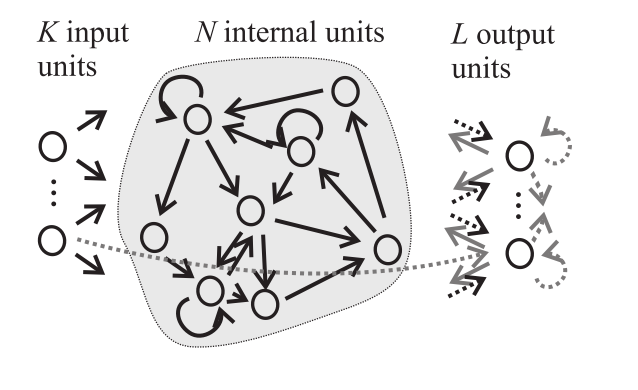
\includegraphics[width=0.8\textwidth]{img/esnG}
	\caption{A basic ESNs architecture taken from \cite{jaeger2001echo}. The network consists
	of three layers, an input layer of size K, an internal reservoir of size N and an output layer of size L.}
\end{figure}

As shown in figure 1, the three different layers in the network have intermediate connections with each other and sometimes they can even have feedback projections onto themselves. The black lines are the necessary connections and the dotted ones are the optional connections. A typical minimal network graph will require three kinds of connections whose weights are expressed as: the input to the reservoir $\mathbf{W^{in}}$ , the internal connections among the units of the reservoir $\mathbf{W}$ and the reservoir to the output units $\mathbf{W^{out}}$. Optional input-to-output connections will increase the performance slightly at the cost of longer training time \cite{davidverstraeten2009} and the optional output feedback loops to the internal units or to the output units themselves are used in signal simulation or to increase memory span\cite{maass2007computational}. For the rest of the discussion, we will stick with the minimal setup with a back projection from output to the internal units, and express the back projection weights as $\mathbf{W^{back}}$.

\paragraph{Propagation steps} At each time step, the internal units are updated using:
\begin{align}
\mathbf{x} (n + 1) = \mathbf{f}(\mathbf{W^{in}u}(n+1) + \mathbf{Wx}(n) + \mathbf{W^{back}y}(n) ) 
\end{align}
$\mathbf{f}$ is the activation functions for the internal units. Threshold functions, hyperbolic tangent functions or sigmoid functions are all candidates for the activation functions. As for the output, we update them using:
\begin{align}
\mathbf{y} (n + 1) = \mathbf{f_{out}}(\mathbf{W^{out}}\mathbf{x}(n+1) ) 
\end{align}

\paragraph{Training steps} We start with some state $\mathbf{x}(0)$ and then use equation (1) to simulate the output signal until $T_{max}$. We then discard the simulation results until $n_{min}$ when, the network dynamics become stable. From this point on, we assume time 0 is the first time step after $n_{min}$. The Error function $E$ usually measures the Mean Square Error (MSE) \nomenclature{\textbf{MSE}}{Mean Square Error} defined as:
\begin{align}
E(\mathbf{y, y^{teach}}) = \frac{1}{N_y} \sum^{N_y}_{i=1} \sqrt{\frac{1}{T} \sum^{T}_{n=1}(y_i(n) - y_i^{teacher}(n) )^2}
\end{align} 
It suffices to run a linear regression on the output signal to minimize the MSE between the predictions and the teacher signals. Nevertheless, after we concatenate the simulation outputs into a matrix $\mathbf{X}$, $\mathbf{X}$ is most likely overdetermined because quite often $ T > N_x $. $N_x$ is the number of the reservoir units. It follows that we need to make use of a few techniques to solve the system. We now look at two of such methods, ridge regression and pseudoinverse inverse.

Ridge regression yields:
\begin{align}
\mathbf{W^{out}} = (\mathbf{y^{teach}X^T(XX^T )} + \beta \mathbf{I})^{-1}
\end{align}
where $\mathbf{I}$ is an identity matrix and $\beta$ is a regularization coefficient. Ridge regression in theory works with large datasets. As shown in equation (4), all the elements do not depend on T. The  limitation of this method is finite floating point representation when one needs to add a big number with a small one \cite{lukovsevivcius2012practical}. Schemes like adding similar values or Kahan summation are recommended \cite{Kahan1965}. 

Pseudoinverse comes to:
\begin{align}
\mathbf{W^{out}} = \mathbf{y^{teach}X^+}
\end{align}
where $\mathbf{X}^+$ is the Moore-Penrose pseudoinverse. This approach is straightforward but the inverse computation is expensive which limits the reservoir size $N_x$ and the number of training data points.

\paragraph{Prediction steps} Implant the trained $\mathbf{W^{out}}$ in the readout layer and do the propagation steps for any new input data. 
 
 \paragraph{Networks parameters} There are three global parameters that define ESNs, namely $(\mathbf{W^{in}, W}, \alpha )$, where $\alpha $ is the rate. There are other important global parameters for the network: the of internal units, sparsity, spectral radius of $\mathbf{W}$ and scaling of $\mathbf{W^{in}}$ \cite{lukovsevivcius2012practical}. To achieve satisfying performance, one should consider the above factors in the design phase. We briefly list a few optimization techniques with respect to those parameters:
 \begin{itemize}
 	\item Spectral radius: The critical parameter that ensures the effectiveness of ESNs. There are a few assumptions that ESNs approach has, one of which is the echo state property. It entails that 
 	\begin{align}
 	\exists E. E = (e_1, \dots, e_N) \text{ where } e_i : U^{-\mathbb{N}} \implies \mathbb{R} 
 	\end{align}
 	so that for any left-infinite input sequence, the current state is determined by:
 	\begin{align}
	\mathbf{x}(n) = \textbf{E}(\dots, \textbf{u}(n - 1), \textbf{u}(n))
 	\end{align}
 	In plain English, the echo state property implies that given a long enough input sequence, the current state is uniquely defined by the previous history such that sequence and the network state $\mathbf{x}(n)$ should not rely on the information that occurs before the initial state the input \cite{jaeger2001echo}. In most cases, $\rho(\mathbf{W}) < 1$ guarantees the echo state property. For the implementation wise, we can first compute the spectral radius of $\mathbf{W}$, and then divide the matrix itself with this value to obtain the unit spectral radius which can be easy to use in the tuning phase.
 	
 	\item Size of the reservoir: In \cite{jaeger2001short}, the memory capacity (MC)  \nomenclature{\textbf{MC}}{Memory Capacity} of an N-unit RNN with linear output to recall an i.i.d. input has been shown to be bounded by N. It makes sense to have $N_x \geq N$ for the minimal setup. On the other hand, only when $T < 1 + N_u + N_x$, will we have a reservoir layer that's too large for the dataset. In general, the bigger the reservoir one uses, the better the performance will be. 
 	 	
 	 \item Leaking rate: The significance of this parameter stems from the discretization of the continuous time update, which can be described as:
 	 \begin{align}
 	 \dot{\mathbf{x}} = -\mathbf{x} + tanh(\mathbf{W^{in}[1; u] + Wx})
 	 \end{align}
 	 where $[-;-]$ represents vector(matrix) wise concatenation. In the context the discrete time, we will have:
 	 \begin{align}
 	 \frac{\Delta\mathbf{x}}{\Delta t} = \frac{\mathbf{x}(n+1) - \mathbf{x}(n)}{\Delta t} \approx \dot{\mathbf{x}} 
 	 \end{align}
 	 It becomes clear that the leaky rate $\alpha$ is the transformation piece between the discrete and continuous worlds. Changing $\alpha$ to match up with the change rate of $\mathbf{u}(n) \text{ and or } \mathbf{y}^{teach}(n)$ is similar to resampling of inputs in order to achieve better performance \cite{schrauwen2007introduction}. 
 	 
 \end{itemize}


\subsection{Resting State Electroencephalogram (EEG)}
EEG measures the electrical activities from the scalp surface which are recorded via electrodes and other conductive media \cite{niedermeyer2005electroencephalography}. The brain has three components: cerebrum, cerebellum and brain stem. EEG is mostly influenced by the activity of the cerebral cortex that is close to the scalp surface. The EEG data records the relative voltage difference between the an electrode and a reference electrode that is usually  being placed in the middle of the scalp. There are two reasons why the raw voltage values are not of interest. First, the voltage values will change due to different choices of baseline subtraction. Secondly, the raw values will be hard to analyze because of the individuals' differences that may not play a role in the desired cognitive processes studies. \cite{cohen2014analyzing}

EEG has three temporal properties: resolution, precision and accuracy. Resolution reflects how many  data points are recorded per unit time, precision reflects how certain the measurements are and accuracy reflects the mapping between the timing of the EEG signals and the timing of the actual occurrences of the events \cite{cohen2014analyzing}. The temporal resolution is determined by the rate of acquisition. It enables one to extract frequency-band-specific features. Furthermore, brain waves are separated into five groups based on their frequency domains. Their corresponding frequency domains are usually associated with:
\begin{itemize}
	\item $  \gamma $ waves: $freq \in (30, 80) Hz$
	\item $ \beta $ waves: $freq \in (13, 30) Hz$
	\item $ \alpha $ waves: $freq \in (8, 13) Hz$
	\item $ \theta $ waves: $freq \in (4, 8) Hz$
	\item $ \delta $ waves: $freq \in (0.5, 4) Hz$
\end{itemize}
The brain waves from different frequency bands look like:

\begin{figure}[h]
	\centering
	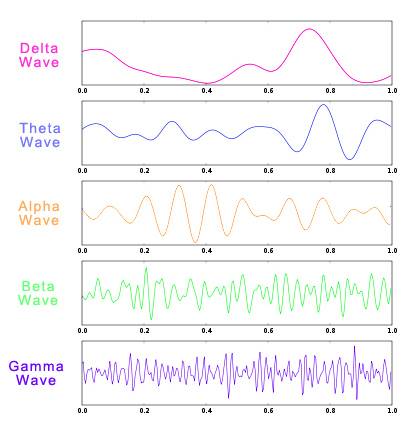
\includegraphics[width=0.5\textwidth]{img/waves}
	\caption[Caption for LOF]{Brain waves visualization based on different frequency bands.\footnotemark}
%	\caption{}
\end{figure}
\footnotetext{Figure taken from the site: http://www.brainworksneurotherapy.com/what-are-brainwaves}
EEG is a good technique to study the brain for a few reasons: This method records the brain dynamics at the time when the cognitive events happen; Secondly, EEG directly measures the brain activity. Changes in voltage potentials are due to neurological behavior at the neuron population level; Lastly, EEG contains rich information and is multidimensional. It not only has the spatiotemporal information, but also frequency, power and phase as features that give us ample knowledge about the internal brain activities. \cite{cohen2011s}

\paragraph{Properties of EEG features for analytics} 
These are paramount factors to consider when one analyzes EEG signals.
\begin{itemize}
	\item Noise and signal: EEG signals are noisy and the noises are often hard to discriminate. One will have to find the fine line between removing too much useful information and having noisy data depending the given task. Figure 3 is a good demonstration of the signal and noise relationship.
	\begin{figure}[h]
		\centering
		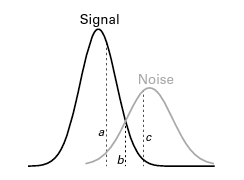
\includegraphics[width=0.5\textwidth]{img/noise}
		\caption{This plot shows the interconnected relationship between signal and noise in EEG (taken from \cite{cohen2014analyzing}). The x-axis is the degree of data cleaning that we conduct and the y-axis is the leftover for signal and noise after the cleaning. We can see the distribution of signal and noise with respect to the level of preprocessing. Area left to a implies there is little noise left, area between a and b has a mixture of both noise and signal and the area right to c has mostly noise.}
	\end{figure}
	\item Non-stationarity: EEG signals can change quickly over time.
	\item Small training sets: Due to the costs of collecting data from subjects, the training sets are oftentimes 
	smaller than ideal.
\end{itemize}

\paragraph{Preprocessing}
\begin{itemize}
	\item Filtering: One wants to have high-frequency artifacts and low-frequency drifts removed in this step.
	It is recommended to use high-pass filter at 0.1Hz or 0.5Hz to get rid of the slow drifts \cite{cohen2014analyzing}.
	\item Spatial filtering: Spatial filtering is needed when you want to localize a result and to eliminate topological features of the data. For instance, if an experiment requires the subjects to conduct some tasks that involve multiple brain regions, it would be otherwise difficult to isolate the active regions without spatial filtering. \cite{cohen2014analyzing}
\end{itemize}

It is worth noting that there is a trend in machine learning that tries to construct end-to-end models without any preprocessing of the data nowadays. People often use a class of techniques called Deep Learning (DL). \nomenclature{\textbf{DL}}{Deep Learning} DL methods compose multiple levels of representational simple and nonlinear layer. Each layer learns at different degrees of abstraction. With enough layers, the models can learn how to discriminate important aspects of data from other variations. DL has made lots of advances in solving challenging problems. In the recent decade, DL has produced competition wining approaches in imaging recognition \cite{krizhevsky2012imagenet}\cite{farabet2013learning} and promising methods for sequence learning tasks in natural language processing \cite{bordes2014question} \cite{luong2014addressing}. However, DL methods are not suitable for EEG data processing, because DL methods usually have many free parameters and it is simply hard to collect enough EEG data for the training purpose. In robotics, although it is also difficult to obtain real world data, people can simulate the training data in a physics engine because the mechanics of robots' interactions and the real world are well understood. Unfortunately, this is not possible for EEG data yet, since we simply don't understand the brain well enough to have a simulator for the brain's underlying mechanisms.


\paragraph{Artifacts}
Artifacts  primarily stem from numerous places in an EEG study, such as blinks, muscle movements and wire noise. Note that EEG is not an error-free measurement technique and we do not know all sources of error. Fortunately after reasonable preprocessing, most analytics tools are robust enough to the noise leftover. Independent Components Analysis (ICA) is the common choice for artifacts removal. It essentially separates the source into different independent sources. Originally, ICA was meant to solve the blind source separation problem, trying to retrieve the independent sources $ \mathbf{s} = ({s_1(t), \dots, s_N(t)})$ \cite{comon1994independent}. The sources $\mathbf{s}$ is being mixed by an unknown matrix $\mathbf{A}$, such that the recorded $N$ mixture $ \mathbf{x} = ({x_1(t), \dots, s_N(t)})$ has the property that 
\begin{align}
\mathbf{x = As}
\end{align} 
ICA in the context of EEG records, separates the data at different electrodes into a sum of various temporally independent components \cite{jung2000removing}, and thus muscle movement, eye blinks and oculomotor activities can generally be detected and rejected. 

\paragraph{Classification overview}
There are five common types of classification algorithms in EEG analytics: linear classifiers, neural networks, nonlinear Bayesian, nearest neighbor and classifiers combinations \cite{lotte2007review}. Here we will discuss two of them and their corresponding characteristics in EEG classification.

\begin{itemize}
	\item Linear classifiers: Linear Discriminant Analysis (LDA) \nomenclature{\textbf{LDA}}{Linear Discriminant Analysis} and SVMs are the most common linear classifiers in EEG analysis. LDA uses several hyperplanes to separate the data. It is cheap to compute and therefore a good candidate for online learning. SVMs also make use of hyperplane separation but they have a different objective, maximizing the margins between different class planes. SVMs have a few good properties, thanks to the regularization terms:  robustness for overfitting and tolerance to the curse-of-dimensionality \cite{bennett2000support}.
	
	\item Neural networks: Multilayer Perceptron (MLP) \nomenclature{\textbf{MLP}}{ Multilayer Perceptron} has been widely used in EEG classification \cite{anderson1996classification}\cite{palaniappan2005brain} due to its flexibility to adapt to different problems. However with noisy and non-stationary data like EEG, it is particularly prone to overfitting \cite{balakrishnan2005multilayer}, and thus it needs careful tuning and architecture design. We should pay special attention to Gaussian classifier which is specifically created to process EEG data in BCIs \cite{millan2004noninvasive} \cite{millan2000local}. In this local neural classifier, each unit in the network is a Gaussian discriminator for each class prototype and if a class has several prototypes, only the nearest one is used. During training, units are pushed towards the EEG samples of the same class and are pushed away from the ones that do not belong to the same class. It has been shown that this kind of architecture is superior to MLP in terms of the rejection efficiency for uncertain samples \cite{millan2000local}. Coming back to ESNs,  they have been used to construct a fast and reliable method for epileptic seizure detection \cite{buteneers2008real}, however, it's not clear how effective ESNs are in EEG classification when being compared with other methods due to the lack of relevant study, nevertheless ESNs should still be a good choice for such a sequence learning task and we would like to explore its limitations in this regard.

\end{itemize}


\section{Motivation}
The main objective of this guided research lies in two folds, one is engineering oriented, and the other is physiology oriented:
\begin{itemize}
	\item Construct a reliable and efficient ESNs to classify the EEG signals.
	\item Explore if there exists a relationship between resting state EEG and MLS. If such a relationship does exist, what we can say about that?
\end{itemize} 

So far the applications of ESNs being used as an EEG classifier is not extensive, although there have been a few in the past years on sequence learning tasks, classifications of real time moving objects \cite{mitul2013classification} and time series classification for the prediction of dialysis \cite{ongenae2013time}. On this note, we wish to summarize the proposed questions of interests from the engineering perspective:
\begin{itemize}
	\item How tolerant ESNs are when dealing with  noisy and non-stationary data like EEG, and when it is good enough to stop cleaning without compromising  useful information.  
	\item How ESNs can best handle time-variant features, more specifically how they deal with the drifting of amplitudes which can be slow and fast at different times?
	\item As training a classifier for EEG using neural networks is prone to over-fitting, what kinds of tuning need to be done in order to avoid this situation?
	\item Is it possible to adapt the reservoir distribution somehow such that the model is better suited for EEG classification?
\end{itemize}

Now we come to the physiological side. So far, stable resting brain activities have been shown to have correlations with personal traits like personality, intelligence and neurological disorder \cite{thatcher2005eeg}\cite{davidson2003affective}. We also know that there is a correlation between event-based computation and the preceding resting state EEG of that event, for instance, the strategy one uses in problem solving \cite{kounios2008origins}. There are more correlations to discover, and correlaton between EEG and MLS is one of them. Merely by using a partial least squares regression model, one can already predict the motor skill acquisition well \cite{wu2014resting}. It would not surprise us if we can achieve better prediction performance using ESNs. Our hypothesis is that the MLS is related to resting state EEG in both young and old age groups. Along with this line of queries, this guided research is determined to tackle the following questions: 

\begin{itemize}
	\item Given the traits of each individual, what is a plausible definition for the MLS that both makes sense physiologically but will also work well for ESNs?
	\item What insights can we learn from the response activity in each internal unit of ESNs? Do the responses contain any critical information about the subjects like the biological age or the cognitive ability?
	\item Does compensation effect exist in old high-performing group?
\end{itemize}

\section{Experiments}
\begin{figure}[h]
	\centering
	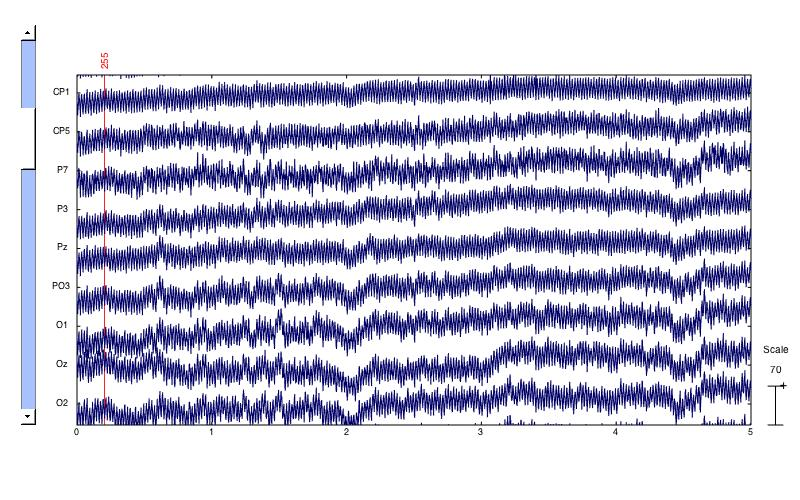
\includegraphics[width=1.0\textwidth]{img/visu}
	\caption{A clip of raw data for 8 channels across five seconds}
\end{figure}


\paragraph{Data source} The EEG data was recorded by Professor Benjamin Godde and his research group for a motor learning study in older adults with 32 channels and at a sampling rate of 2048 Hz. In figure 4, one can see a short clip for the EEG recording for eight channels. Clearly, most of the signals demonstrate some periodic behaviors and on the lower half of the plot, channels like O1, Oz and O2 have more fluctuations within this time frame.  The recording machinery is an active electrode system (ActiveTwo, BioSemi, Amsterdam, Netherlands) mounted in an elastic nylon cap \cite{jasper1958ten}. The eventual usable data contains 79 subjects' resting EEG recordings for 80 seconds. There are 30 young subjects and 49 old subjects. The total EEG data is about 1.5 GB. In addition, for each subject, we have a few meta variables, some of which are going to compose MLA later on:
\begin{itemize}
	\item Biological traits: age and gender
	\item Age group: a binary class variable to denote if a participant belongs to the young or old group
	\item Moca: an indicator value for the risk of dementia
	\item $VO_2$ peak: peak oxygen consumption in a stationary bicycle task for fitness level measurement
	 \item MVC: max voluntary contraction, the max force between the thumb and index finger for 5 seconds 
	 \item PreRMSE and PostRMSE: the motor performance before and after the motor learning training
\end{itemize}

Since we are building a binary EEG classifier, the model construction pipeline is quite obvious. For this project, we follow the construction diagram in Figure 5. The whole experiment section mainly consists three stages: preprocessing, model building and post-processing.

\begin{wrapfigure}{l}{0.5\textwidth}
	\begin{center}
		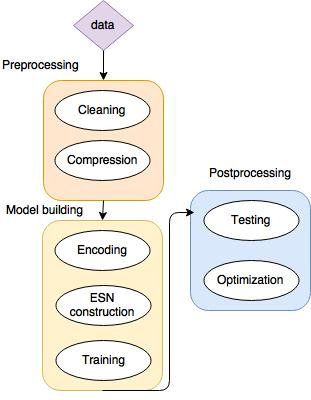
\includegraphics[width=0.40\textwidth]{img/dataflow}
	\end{center}
	\caption{Data processing pipeline}
\end{wrapfigure}

	\paragraph{Preprocessing} As we already discussed in section 4, two of the main problems that an EEG classifier faces are the curse of dimensionality and low data-noise ratio. Therefore, cleaning and compression stages are necessary. For cleaning, we use a bandpass filter 0.5 - 79 Hz. The artifacts are not removed in this project because firstly, manual inspection of ICA component for artifacts removal requires domain expertise, and secondly, automation of artifact removals in EEG is another research question and is non-trivial on itself. Furthermore, we normalize each input channel by 
	$$ \bar{u}_i(t) = \frac{u_i(t) - mean(u_i)}{max(u_i) - min(u_i)} i \in [1, 12] $$
	   In addition, we remove the subjects whose EEG recordings are strongly influenced by artifacts and prior caffeine intake. Finally, we get rid of the relative MLS outliers which leaves us with 77 training samples.
		
	In the compression stage, we choose only 12 electrodes (F3 C3 P3 Pz O1 Oz O2 P4 C4 F4 Fz Cz) because  there are overlaps among electrode recordings. The exact locations of these electrodes on the scalp are shown in figure 6. Then we will down sample the frequency from 1024 Hz to 512 Hz. Recordings at extremely high frequencies do not have the relevant information about brain processes. We denote each electrode's recording by $c_i. i \in [1, 12]$. 
	
	Lastly, in preparation for the  cross-validation, we split all the subjects into 5 groups. During the testing phase, we will just leave out one group for testing in each iteration. In figure 7, we can see a five-second clip of the preprocssed EEG sample. The pattern of the signal is more clear and less dense as compared to the raw form shown in figure 4. All the preprocessing is done in Matlab using EEGLAB toolbox \cite{delorme2004eeglab}.
	\begin{figure}[!h]
		\begin{center}
			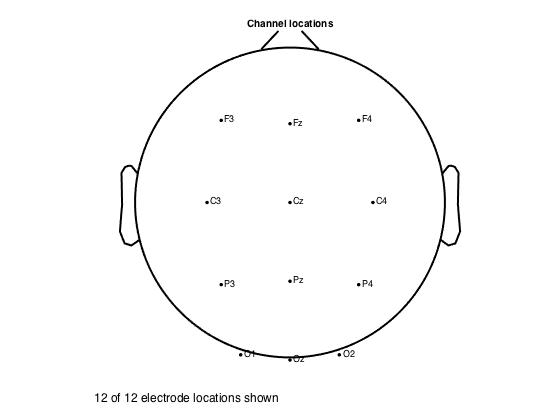
\includegraphics[width=0.7\textwidth]{img/chanLocation}
		\end{center}
		\caption{Locations of 12 selected electrode channels.}
	\end{figure}
			\begin{figure}[!h]
	\begin{center}
		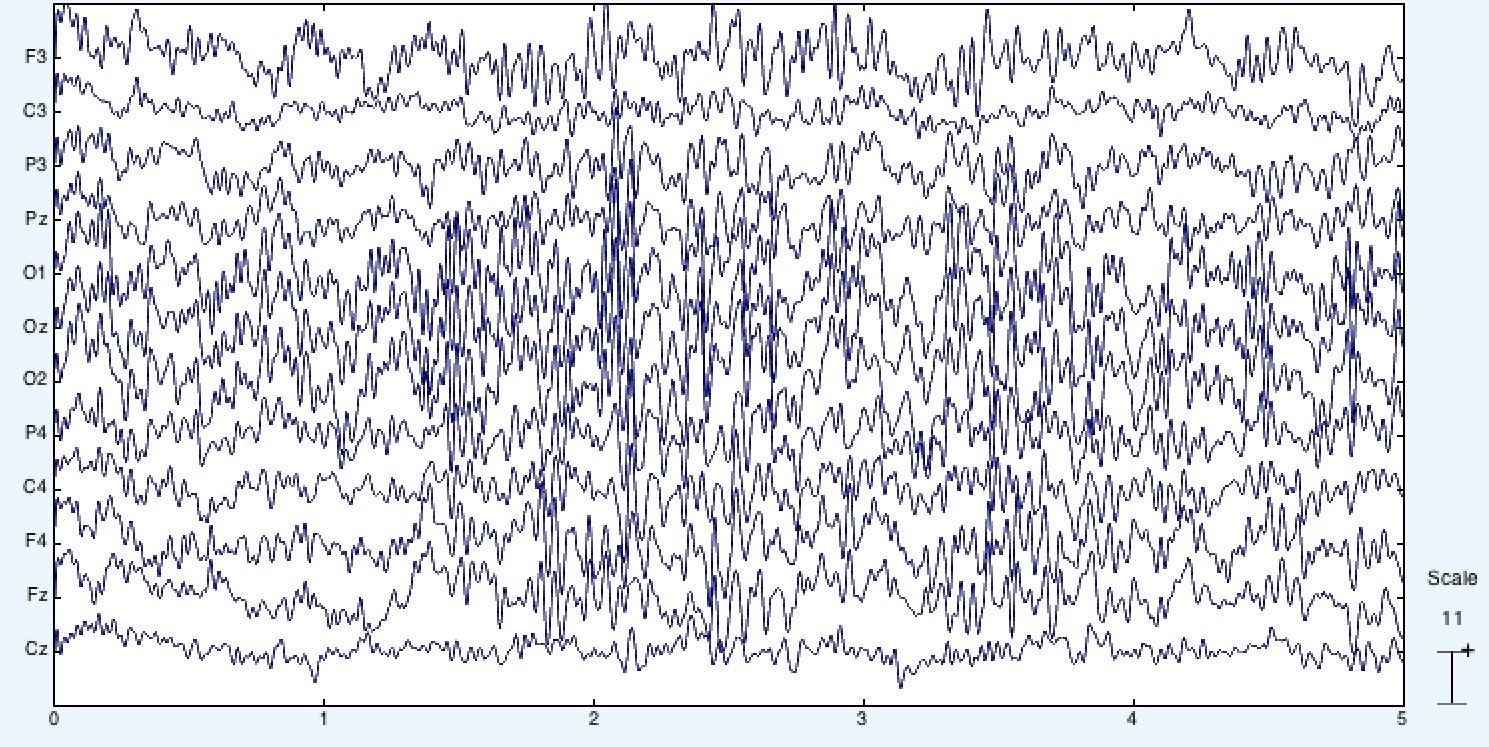
\includegraphics[width=0.9\textwidth]{img/processed}
	\end{center}
	\caption{Preprocessed EEG sample.}
	\end{figure}

\paragraph{Model Building} 

\begin{itemize}
	\item Encoding : After finished preprocessing the data, we define the relative MLS as $$ MLS = \frac{PreRMSE - PostRMSE}{PreRMSE}  $$
	The relative MLS is the main criterion that we use to label the subjects.   
	In figure 8, we have the age (y axis) versus relative MLS (x axis) scatter plot.  For the relative MLS, the smaller the value is, the more one's motor skills can improve after training. We have three groups of subjects: yellow dots old high performing, blue dots old low performing and purple dots young high performing. All young subjects are considered high performing and among the old subjects, we use the median to differentiate the high performing and low performing subjects.
	
	\item ESN construction:  We start by using a network of 100 reservoir units and try out unit size of 150 and 250. We also use leaky neurons to update. Then we construct the teacher signal, a vector of size two by one, one element being one and the other being zero depending on which MLS group this subject belongs to. In the predication phase, we first exploit the inputs $\mathbf{u}$ by using the updates rules defined in equation (2), and obtain $\hat{\mathbf{y}}$ of size 2 by T. The class of $\mathbf{u}$ thus becomes:
	$$ class_{idx} = max_{rowidx} \frac{\sum_i^T\mathbf{y_{1i}}}{\sum_i^T\mathbf{y_{2i}}} $$
	
	\item Training: We use the ridge regression with regularization which is discussed in section 2.1. In our experiment we train three binary classifier in total: young high performers vs old high performers, young high performers vs old low performers and old high performers vs old low performers.
	
\end{itemize}
\begin{figure}[h]
	\centering
	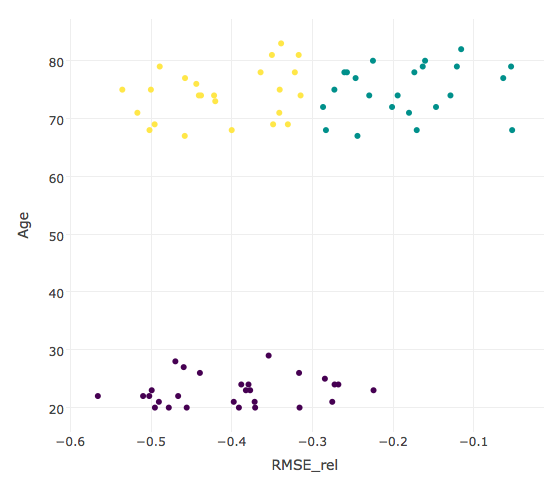
\includegraphics[width=0.6\textwidth]{img/scatter}
	\caption{The scatter plot of age vs the relative motor training improvement is shown. The y-axis is for age and the x-axis is for the relative motor training improvement. The smaller the x value is, the more one has improved after motor training. Yellow dots are old high performers; blue dots are old low performers; purple dots are young high performers.}
\end{figure}

\paragraph{Post-processing}
As we know, EEG classification is prone to over-fitting, so after the model's been constructed, we fine tune  washout threshold, spectral radius, regularization and the leaking rate to get better results \cite{lukovsevivcius2012practical}. These four parameters are mostly dealt with and the other parameters are disregarded in this experiment.

\section{Results}
\paragraph{Stratified five-fold cross-validation}
In the evaluation phase, we use stratified five-fold cross-validation. Conventional cross-validation in our experiment setup wouldn't work well because we only have two classes and a small number of samples in the order of tens, and therefore in the cross-validation phase mere random allocation of the data samples to different folds might lead to a situation where one class is only present in the testing but not in the training phase which will surely leads to bad performance. A good evaluation method should have both low bias and low variance and k-fold stratified cross-validation is general better than the regular version \cite{kohavi1995study}. We only have 77 subjects and three groups but we are constructing three mutual binary classifiers among these groups, which gives fewer data points. Hence we use the stratified five-fold cross-validation scheme to evaluate the model results.

\paragraph{Parameter selection}
The washout threshold stays reasonably stable when other parameters are changing so we pick the washout threshold first. The deciding factor is when we move back the threshold, the classification result doesn't fluctuate too much, and at the same time that the internal neuron responses remain relatively stable. The first value of such a point should be the washout threshold. in our experiment, we found out 550 is a good enough washout threshold.

The parameter values for the young high performers vs old low performers and young high performers vs old high performers are quite similar so we just showcase the validation error behavior on the young high performers vs old low performers model. 

\begin{figure}[h]
	\centering
	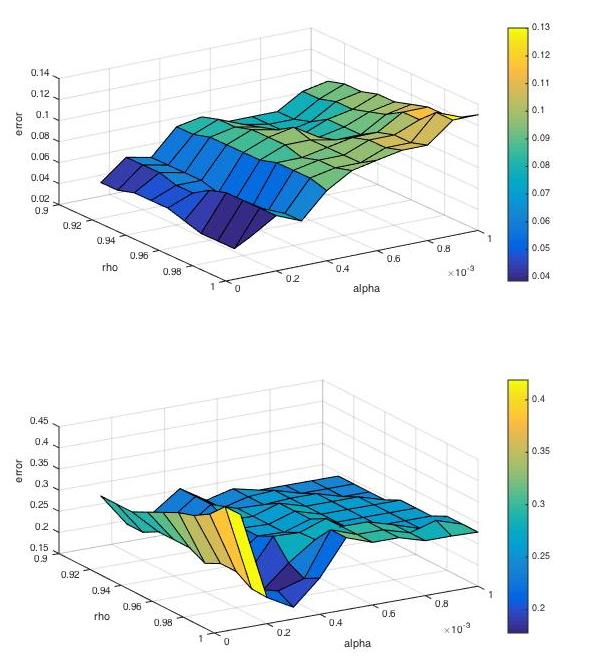
\includegraphics[width=0.7\textwidth]{img/pair}
	\caption{The top is the training error and the bottom is the testing errors with respect to the leaky rate and the spectral radius for young high performers vs old low performers.}
\end{figure}
After washout threshold is being set, we first do a sparse parameters manual search to locate the range of the values to do a systematic tunning, then we do a grid search on two of the parameters. In this case we do a grid search with respect to the leaky rate $\alpha$ and the spectral radius $\rho$.  In figure 9, the training error declines when either $\alpha$ or $rho$ declines, whereas the testing error has a local minimum when $\alpha = 0.0003$ and $ \rho = 1$ with a training error at 0.0627 and testing error at 0.1776. 

Now we can fix the $\alpha$ and $\rho$ to do a single for loop on regularization coefficient:  
\begin{figure}[h]
	\centering
	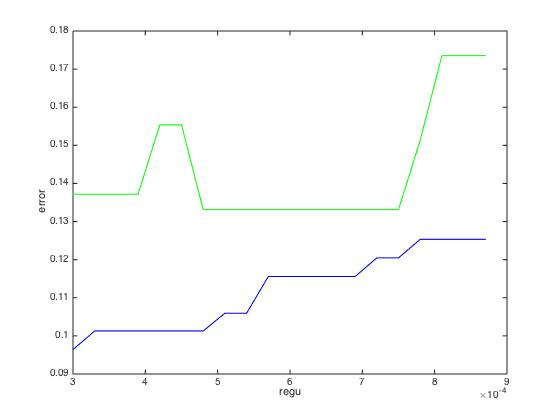
\includegraphics[width=0.7\textwidth]{img/regu}
	\caption{Error behavior when $\alpha = 0.0003$ and $ \rho = 1$ with respect to regularization coefficient.}
\end{figure}
So the training keeps increasing when regularization coefficient climbs up and the minimum of testing error hits when the coefficient is between 0.0005 and 0.00075. The testing error is around 0.1331 and the min training error across this range is 0.0964. The classifier of young high performers vs old high performers can also achieve 0.1331 using similar set of parameters.

The author could not find a set of good parameters to make the old high performers vs old low performers classifier do better than random chance, and thus the error plots of that model is not included. 


\begin{table}[h!]
	\centering
	\begin{tabular}{||c c c||} 
	\hline
	Model Name & Training error & Testing error \\ [0.5ex] 
	\hline\hline
	Old high performers vs young high performers & 0.1205 & 0.1331 \\ 
	\hline
	Old low performers vs young high performers & 0.0964 & 0.1331 \\ 
	\hline
	Old low performers vs old high performers & 0.1965 & worse than random chance \\ [1ex] 
	\hline
\end{tabular}
\caption{Table for training and testing errors. The third model's training error was the taken from the best trial across all tested parameters regardless the testing error.}
\end{table}

\todo{add confusion matrix for both models}


\section{Discussion}


\section{Conclusion}

\clearpage
\newpage

\bibliographystyle{unsrt}
\bibliography{thesis}

\end{document}
